
%\documentclass[english]{ipsj}
%\documentclass[english,preprint]{ipsj}
\documentclass[english,preprint,JIP]{ipsj}

\usepackage{graphicx}
\usepackage{latexsym}
\usepackage{algorithm}
\usepackage{algpseudocode}
\usepackage{enumitem}
\usepackage{tikz}
\usepackage{url}
\usetikzlibrary{positioning}


\newcommand{\maru}[1]{\raise0.2ex\hbox{\textcircled{\scriptsize{#1}}}}

\def\Underline{\setbox0\hbox\bgroup\let\\\endUnderline}
\def\endUnderline{\vphantom{y}\egroup\smash{\underline{\box0}}\\}
\def\|{\verb|}


\setcounter{volume}{26}% vol25=2017
\setcounter{number}{1}%
\setcounter{page}{1}


\received{2016}{3}{4}
%\rereceived{2011}{10}{1}   % optional
%\rerereceived{2011}{10}{31} % optional
\accepted{2016}{8}{1}



\usepackage[varg]{txfonts}%%!!
\makeatletter%
\input{ot1txtt.fd}
\makeatother%

\begin{document}

\title{Cantata: Accelerating Aria with Early Dependency Resolution}

\affiliate{KU}{Keio University, Kanagawa, Japan}
\affiliate{CL}{Cybozu Labs, Tokyo, Japan}

\author{Yusuke Miyazaki}{KU}[miyayu@keio.jp]
\author{Takashi Hoshino}{CL}[hoshino@labs.cybozu.co.jp]
\author{Hideyuki Kawashima}{KU}[river@sfc.keio.ac.jp]


\begin{abstract}
Aria is a deterministic concurrency control protocol designed for long-running and highly contended transaction processing workloads.
Although Aria achieves high performance by concurrently executing conflicting transactions, its all-at-once dependency checking causes unnecessary aborts and redundant operations, leading to inefficiency under high contention.
To address this issue, this paper proposes a novel optimization called early dependency resolution.
The proposed method divides Aria's dependency checking into two stages: the first stage checks only write-after-write dependencies, while the second stage checks the remaining read-after-write and write-after-read dependencies.
By early aborting in the first stage, the second stage can skip redundant read reservations and reduce unnecessary aborts.
Consequently, the proposed method expands the scheduling space beyond that of vanilla Aria and improves performance.
We implemented the proposed method on the open-source implementation of Aria and compared it with vanilla Aria.
The results show that the proposed method outperforms vanilla Aria under high-contention and long-running workloads, achieving up to a 2.4x throughput improvement in realistic YCSB settings.
Furthermore, a controlled experiment that isolates the cost of redundant read reservations confirms the core mechanism, yielding up to a 774x speedup.
\end{abstract}

\begin{keyword}
concurrency control, deterministic protocol, Aria, early dependency resolution, transaction processing
\end{keyword}

\maketitle

%1
\section{Introduction}
\subsection{Motivation}
Concurrency control protocols are key components of transaction processing. When multiple transactions access the database simultaneously, the data accesses must be serialized so that they never result in inconsistent states called anomalies~\cite{weikum2001}. To maintain the integrity and consistency of the database, concurrency control protocols determine which transactions to abort and which to commit. To accelerate concurrency control, a variety of protocols have been proposed. They can be mainly categorized into deterministic~\cite{calvin,lu2020aria,thomson2010case,faleiro17,nemoto2022oze} or non-deterministic~\cite{nakamori2022decentralization, tu2013speedy, ermia, yu2016tictoc, lim2017cicada}.  %pessimistic~\cite{nakamori2022decentralization}, optimistic~\cite{tu2013speedy} or multi-versioning~\cite{ermia}. 

Classical non-deterministic approaches perform well in relatively short transaction workloads such as YCSB or TPC-C~\cite{ccbench,abyss,Bang20}. However, they do not exhibit sufficient performance in long-running transaction workloads like the bill of materials or graph processing~\cite{nemoto2022oze,mammoth} because such transactions can encounter many conflicts, and one of the conflicting transactions must be aborted.
%
To address the problem, the deterministic approach~\cite{calvin, thomson2010case, qin2021caracal, faleiro17} has been studied. 
%
Since deterministic protocols determine the order of transaction execution for a set of transactions in the first phase, they do not need to abort transactions. 
%
Aria~\cite{lu2020aria} is one of the fastest deterministic protocols. Conventional deterministic protocols execute transactions individually and serially if they conflict, in order to provide deterministic results. Aria, however, executes transactions concurrently even if they conflict. This concurrent execution approach, combined with sophisticated optimization methods, offers high performance. 
%
The motivation for this work is to further accelerate Aria by addressing its remaining inefficiency in dependency checking.

\begin{figure}[tb]
\centering
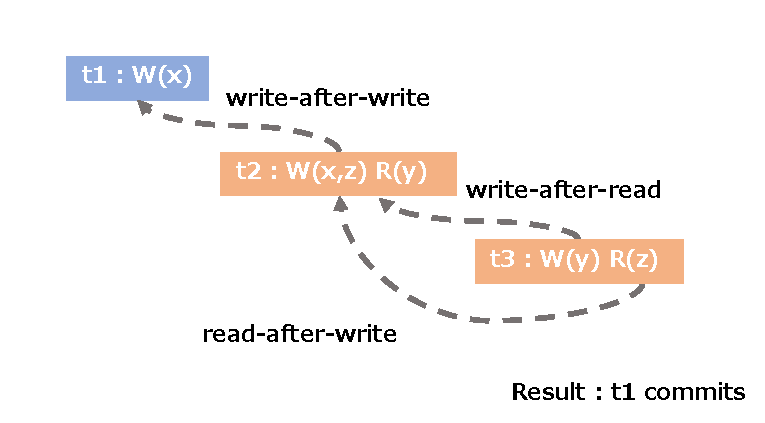
\includegraphics[width=0.95\linewidth]{figures2/problem1.pdf}
\caption{The unnecessary abort of $t_3$ caused by $t_2$.}
\label{fig:problem}
\end{figure}


\subsection{Problem}

Aria processes transactions in batches like other deterministic concurrency control protocols, 
with transactions in the same batch performing reads against the same database snapshot.
%
Aria determines which transactions to abort by examining three types of dependencies---Write-after-Write (WAW), Read-after-Write (RAW), and Write-after-Read (WAR)---between concurrent transactions.

Figure~\ref{fig:problem} illustrates the problem through a running example with three concurrent transactions $t_1$, $t_2$, $t_3$ in a batch. In this example, $t_2$ is aborted due to a WAW dependency with $t_1$. However, because Aria checks all three dependencies simultaneously, $t_3$ is also unnecessarily aborted due to its dependencies on the already-aborted $t_2$. This unnecessary abort shrinks Aria's scheduling space and degrades performance. We elaborate on the technical cause of this problem in Section~\ref{sec:problem_aria}.

\begin{figure}[tb]
\centering
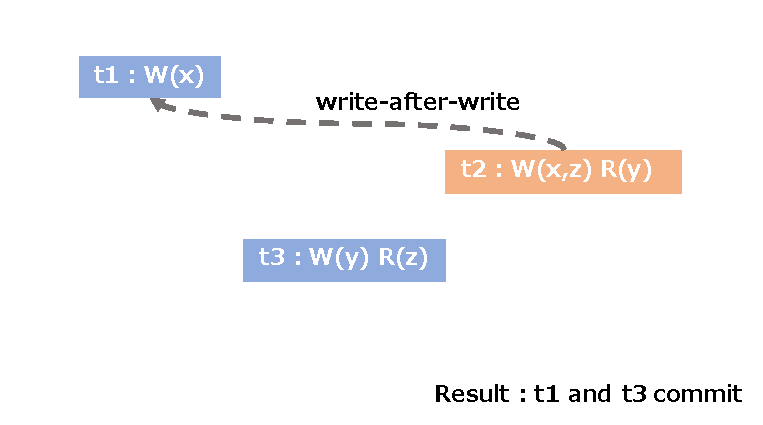
\includegraphics[width=0.95\linewidth]{figures2/solution1.pdf}
\caption{$t_3$ does not observe the operations of the aborted $t_2$.}
\label{fig:solution}
\end{figure}

\subsection{Contribution}

The unnecessary aborts stem from the coarse-grained handling of dependencies. 
If we could immediately abort $t_2$ in Figure~\ref{fig:problem}, the abort of $t_3$ would not occur.
This is impossible in Aria because it checks WAW, WAR, and RAW dependencies altogether only at the end of the execution phase.

This paper proposes an optimization method to address this problem. 
Our idea is \textbf{early dependency resolution}. It divides the execution phase into two stages.
The first stage checks only WAW dependencies, and the second stage checks WAR and RAW dependencies. 
%
The proposed method excludes the reads and writes of transactions aborted by the WAW dependency for the confirmation of WAR and RAW dependencies. 
%
Thus, in situations like the one shown in Figure~\ref{fig:problem}, $t_3$ can ignore the reads and writes of $t_2$, allowing both $t_1$ and $t_3$ to commit. In addition, if a transaction such as $t_2$ is known to fail due to a WAW dependency, subsequent operations can be skipped, reducing unnecessary overhead.
As a result, the proposed method does not abort $t_3$ as shown in Figure~\ref{fig:solution}. 

We implemented the proposed method on the open-source implementation of Aria and compared it with vanilla Aria. 
The experimental results showed that the proposed method achieved up to a 2.4x throughput improvement in realistic YCSB settings, and a controlled experiment that artificially amplifies the cost of redundant operations confirmed up to a 774x speedup.

\subsection{Organization}
The rest of this paper is organized as follows.
Section 2 describes deterministic protocols and Aria as the preliminaries.
Section 3 describes the proposed method, early dependency resolution.
Section 4 describes the evaluation of the proposed method.
Section 5 describes related work.
Section 6 concludes this paper.

\section{Preliminaries}
\subsection{Deterministic Protocol}
Concurrency control protocols can be classified into two types based on their nature: deterministic concurrency control~\cite{calvin, faleiro17, qin2021caracal, thomson2010case} and non-deterministic concurrency control~\cite{yu2016tictoc,tu2013speedy,nakamori2022decentralization}. 
%
Aria, discussed in this paper, is one of the deterministic concurrency control protocols. 
A deterministic protocol first collects a set of transactions and then executes them. The results of transactions are always the same even if they are executed multiple times. Thus, deterministic protocols are amenable to distributed transaction processing systems that provide fault tolerance~\cite{calvin}. 

To provide determinism, in most deterministic protocols, transactions in a set are executed one by one if they conflict with one another~\cite{thomson2010case,calvin,qin2021caracal,faleiro17}.
Aria~\cite{lu2020aria} is different from such classical protocols. It concurrently executes a set of transactions even if they are conflicting. 

%%%%%%%%%%%%%%%%%%%%%%%%%%%%%%%%%%%%%%%%%%%%%%%%%%%%%
\subsection{Aria}
The processing flow of Aria is shown in Figure~\ref{fig:aria}. 
In Aria, every transaction is assigned a unique transaction identifier (tid) and grouped into batches through a sequencing layer. These batches go through the execution phase and the commit phase. 

In the execution phase, transactions within a batch perform read operations over the same database snapshot and create local read and write sets in their own memory space. 
%
Each transaction also performs read and write reservations, attempting to reserve the data items in its read and write sets. Write reservations are only successful if a transaction with a smaller tid has not already reserved the data item. Otherwise, the transaction will abort at the subsequent commit phase.
Read reservations work in the same way, but they use the read set instead.

Once all transactions in a batch complete the execution phase, they immediately move on to the commit phase.
%
During the phase, each transaction checks for three types of dependencies (WAW, RAW, and WAR) by referring to the reservations made for the data in its local write and read sets. Note that transactions cannot enter the commit phase until all transactions in the batch have completed the execution phase.
%
These dependencies are defined as follows, where $i$ and $j$ are any two tids with $i < j$:
\begin{enumerate}
    \item When $t_i$ and $t_j$ both write to the same data item, $t_j$ is said to have a WAW dependency on $t_i$.
    \item When $t_j$ reads a data item written by $t_i$, $t_j$ is said to have a RAW dependency on $t_i$.
    \item When $t_j$ writes to a data item read by $t_i$, $t_j$ is said to have a WAR dependency on $t_i$.
\end{enumerate}

In Aria, a transaction $t_j$ can commit if it satisfies the following two conditions:
\renewcommand{\labelenumi}{\alph{enumi})}
\begin{enumerate}
    \item There is no $t_i$ in the batch with which $t_j$ has a WAW dependency.
    \item Transaction $t_j$ does not simultaneously have WAR and RAW dependencies in the same batch.
\end{enumerate}

\begin{figure}[tb]
\centering
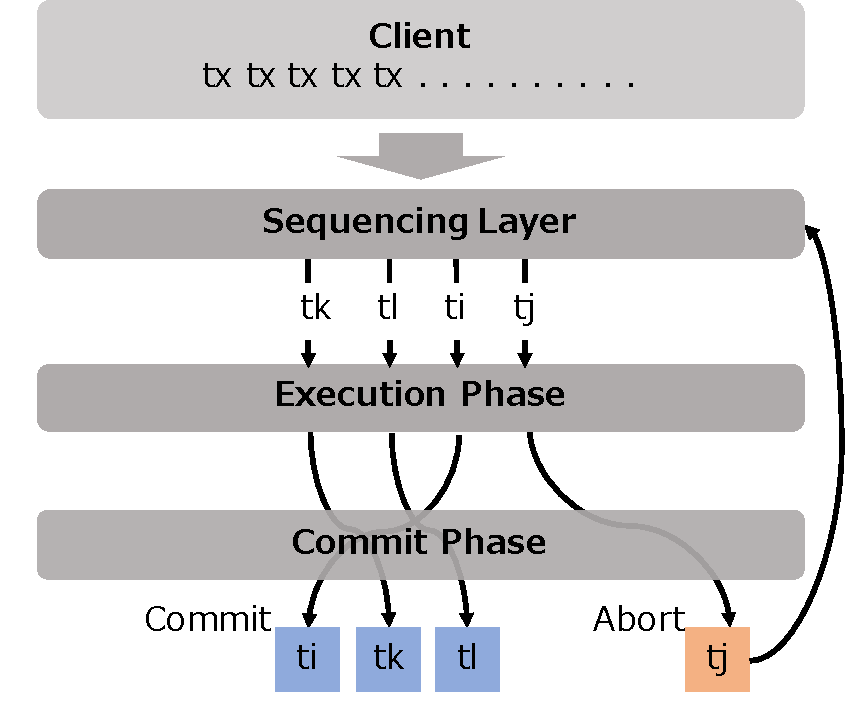
\includegraphics[width=0.75\linewidth]{figures2/ariaflow.pdf}
\caption{The flow of transaction processing in Aria. After collecting a set of transactions at the sequencing layer, transactions are concurrently executed in the execution phase.}
\label{fig:aria}
\end{figure}

\subsection{Problem of Aria}
\label{sec:problem_aria}
As shown in Figure~\ref{fig:aria_method}, Aria manages conflict relationships using a table. 
The attributes of the table are the write tid and the read tid. Each record represents the conflict relationship for a single data item.
The figure illustrates three transactions $t_1$, $t_2$, $t_3$ in a batch. 
%
Here, $t_2$ is aborted due to a WAW dependency with $t_1$ because it performs a write operation on data item x, which is already written by $t_1$.
%
$t_3$ reads data item z, which is written by $t_2$, creating a RAW dependency, and writes to item y, which is read by $t_2$, creating a WAR dependency. Regarding condition b), since $t_3$ has both a WAR dependency and a RAW dependency on $t_2$, it aborts. 
%
The problem is that this abort of $t_3$ is unnecessary: $t_2$ is already aborted due to a WAW dependency, and thus the dependencies between $t_2$ and $t_3$ should vanish. However, Aria performs write and read reservations for all transactions, including those aborted due to WAW dependencies, and then checks for WAR and RAW dependencies all at once. As a result, Aria can produce false positives~\cite{weikum2001}.

%%%%%%%%%%%%%%%%%%%%%%%%%%%%%%%%%%%%%%%%%%%%%%%%%%%%%%%%%%%%

\section{Early Dependency Resolution}
\subsection{Optimization Method}
To address the limited scheduling space caused by Aria's simultaneous dependency checking, we propose a novel optimization method called \textbf{early dependency resolution} for Aria. 
%
By resolving dependencies early, Aria can avoid unnecessary aborts and redundant reservation processing.
%
Hereafter, we refer to Aria augmented with this optimization as \textbf{Cantata}.
%

Cantata separates the dependency checking into two stages to eliminate the false positives caused by simultaneous checking. 
%
First, each transaction creates its local read and write sets as in vanilla Aria. 
Each transaction then performs write reservations to detect WAW dependencies. 
%
At the end of this stage, conflicting transactions are immediately aborted, which constitutes the key distinction from vanilla Aria. This immediate abort expands the scheduling space.
%

Second, only those transactions that are not aborted by WAW dependencies in the first stage can perform read reservations and check for WAR and RAW dependencies. Vanilla Aria checks all three dependencies simultaneously, whereas Cantata does not need to recheck WAW dependencies in this stage.
%
%In the dependency checking, write reservations of aborted transactions due to WAW dependencies are ignored.
%Since the abort of a transaction is determined at the second stage

\subsection{Running Example}
We show a running example of the behavior of Cantata in Figure~\ref{fig:ariaER_method}.
%
As transactions execute, their transaction IDs (tid) are recorded in the $write\_tid$ and $read\_tid$ columns of each data item for write and read reservations, respectively.
%
First, in \maru{1}, transactions $t_1$, $t_2$, and $t_3$ make write reservations. 
%
Each transaction then checks if it has a WAW dependency. In the situation shown, $t_1$ successfully makes a write reservation for data item x that $t_2$ is also trying to write to. 
%
Thus, $t_2$ has a WAW dependency on $t_1$ and is aborted. Meanwhile, $t_3$'s write reservation on item y succeeds because no other transaction with a smaller tid writes to y; hence $t_3$ has no WAW dependency and survives this stage.
%
Next, in \maru{2}, read reservations are made by transactions that were not aborted due to WAW dependencies, and WAR and RAW dependencies are checked. At this point, since $t_2$ is already recorded as WAW-aborted in the abort list, its reservations are ignored during dependency checking. Therefore, $t_3$ disregards $t_2$'s write reservation on item z and has no RAW dependency. Similarly, $t_2$'s read reservation on item y is also disregarded, so $t_3$ has no WAR dependency either. As a result, $t_3$ commits successfully.

%%%%%%%%%%%%%%%%%%%%%%%%%
\begin{figure}[tb] 
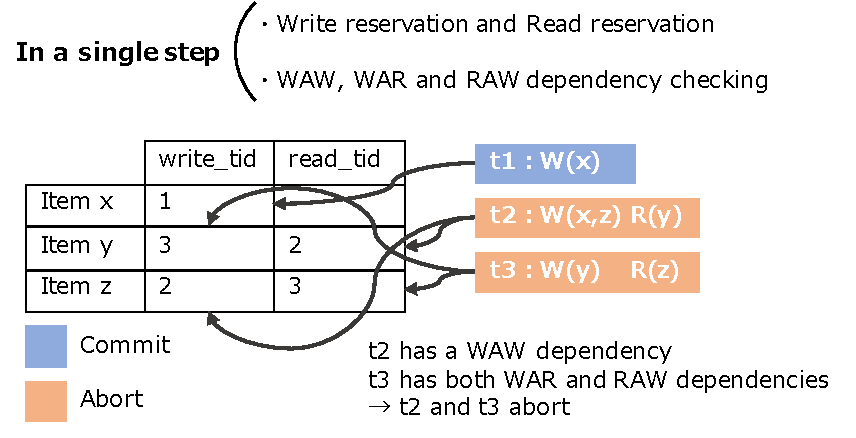
\includegraphics[width=\linewidth]{figures2/ariamethod.pdf}
\caption{Data structures for Aria. The table, abort list, maintains dependencies between transactions for each data item in the database. $t_1$ writes to item-x/write\_tid, subsequent $t_2$ cannot overwrite it since its tid is larger than that of $t_1$.} 
\label{fig:aria_method} 
\end{figure}

Implementing Cantata requires managing the reservations of transactions aborted due to WAW dependencies. Two approaches are possible: (1)~having the aborted transactions directly remove their reservations, or (2)~having each surviving transaction validate reservations during dependency checking. We adopt the second approach because the first requires an additional synchronization barrier between the two stages, which would degrade performance due to thread synchronization overhead.

The proposed method uses a data structure called the \emph{abort list} to record transactions aborted due to WAW dependencies. As shown in Figure~\ref{fig:list}, the abort list is an array with one slot per transaction in a batch. Each slot stores a generation value, and a global generation counter $g$ is incremented at the beginning of each batch. When a transaction is aborted due to a WAW dependency, its slot is set to the current generation $g$; a transaction is considered WAW-aborted if and only if its slot matches $g$. This design eliminates the need to reset the array between batches, since slots from previous batches naturally hold stale generation values.
Because the generation counter is incremented only once per batch and each abort-list lookup reduces to a single integer comparison, the per-transaction overhead of maintaining this structure is minimal.
During RAW checking, the corresponding abort-list entry of a writer is identified from the writer tid stored in the metadata.

\subsection{Algorithm}
The details of Cantata are presented in Algorithms~\ref{alg1},~\ref{alg2}, and~\ref{alg3}. Algorithms~\ref{alg1} and~\ref{alg2} define the subroutines for reservation and dependency checking, corresponding to \maru{1} and \maru{2} in Figure~\ref{fig:ariaER_method}, respectively. Algorithm~\ref{alg3} describes the overall batch processing flow that invokes these subroutines, including the elimination of WAW-aborted transactions.

\begin{figure}[tb] 
\centering
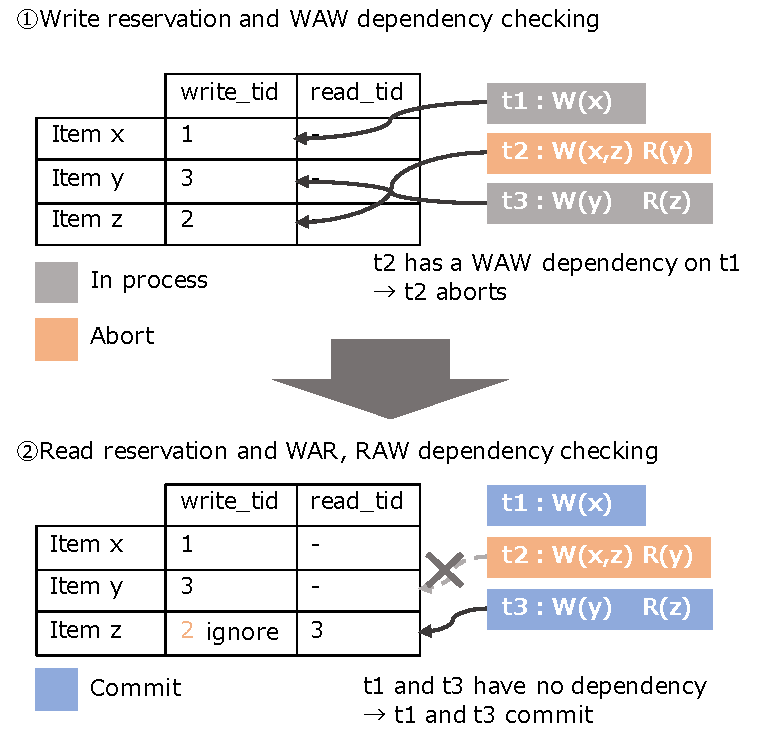
\includegraphics[width=0.95\linewidth]{figures2/edrmethod.pdf}
\caption{Behavior of Cantata. $t_2$ detects a WAW dependency with $t_1$ when it checks item x/write\_tid. Since $t_2$ is recorded as WAW-aborted, its reservations are ignored during subsequent dependency checking. Thus, $t_3$ is not affected by $t_2$.} 
\label{fig:ariaER_method} 
\end{figure}


\begin{figure}[tb]
\centering
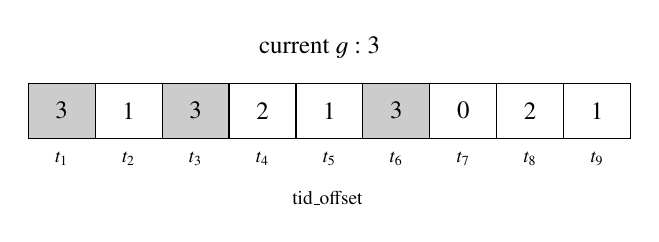
\begin{tikzpicture}[
    slot/.style={draw, minimum width=0.85cm, minimum height=0.7cm, font=\small},
    aborted/.style={slot, fill=black!20},
]
\foreach \i/\g/\st in {0/3/aborted, 1/1/slot, 2/3/aborted, 3/2/slot, 4/1/slot, 5/3/aborted, 6/0/slot, 7/2/slot, 8/1/slot} {
  \node[\st] (s\i) at (\i*0.85+0.425, 0) {\g};
}
\foreach \i in {0,...,8} {
  \node[font=\scriptsize, below=1pt of s\i] {$t_{\the\numexpr\i+1}$};
}
\node[font=\small] at (3.7, 0.8) {current $g{\ :\ }3$};
\node[font=\scriptsize, below=0.55cm] at (3.8, -0.35) {tid\_offset};
\end{tikzpicture}
\caption{Structure of the abort list. Each transaction in a batch has one slot that stores a generation value (gen). A transaction is WAW-aborted if and only if its slot matches the current generation $g$. Shaded slots indicate aborted transactions ($t_1$, $t_3$, $t_6$).}
\label{fig:list}
\end{figure}

As shown in Algorithm~\ref{alg3}, processing begins with the execution phase, in which each transaction creates local read and write sets against the database snapshot and performs write reservations via \texttt{ReserveWrite()} (Algorithm~\ref{alg1}). A barrier then ensures that all write reservations are complete before proceeding.

In the commit phase, Stage~1 checks for WAW dependencies using the \texttt{WAW()} function (Algorithm~\ref{alg1}). When a transaction aborts due to a WAW dependency, it records this fact by writing the current generation to the corresponding slot in the Abort List.

In Stage~2, only transactions not marked in the Abort List perform read reservations via \texttt{ReserveRead()} (Algorithm~\ref{alg2}). A second barrier ensures that all read reservations are complete. Then, in Stage~3, the remaining transactions check WAR and RAW dependencies using \texttt{WAR()} and \texttt{RAW()} (Algorithm~\ref{alg2}). During the \texttt{RAW()} check, for each data item in the transaction's read set, the \textsc{WriterOffset} function maps the tid of the transaction that wrote to that item to its abort-list entry; if that writer has been recorded in the Abort List, the write reservation is ignored.

Finally, in Stage~4, each transaction is committed or aborted: transactions marked in the Abort List are aborted, and among the remaining transactions, those that have both WAR and RAW dependencies are also aborted. All other transactions commit and apply their write sets to the database. After a final barrier, the next batch begins, and aborted transactions are re-executed in the subsequent batch.

\begin{figure}[!t]
\begin{algorithm}[H]
    \caption{First dependency check in Cantata}
    \label{alg1}
    \begin{algorithmic}[1]  
    \Require Transaction $Tx$ with read set $Tx.RS$, write set $Tx.WS$, transaction id $Tx.TID$, epoch $Tx.Epoch$, abort-list entry $Tx.Offset$; current generation $g$
    \Statex Each $\textit{Table}$ entry stores an epoch together with $write\_tid$ and $read\_tid$. Reservations from previous batches are ignored unless the stored epoch matches $Tx.Epoch$.
    \State
    \Function{ReserveWrite}{$Tx$}
        \For{each $key$ in $Tx.WS$}
            \State Acquire $\textit{Table}[key].lock$
            \If{$\textit{Table}[key].epoch < Tx.Epoch$}
                \State Reset $\textit{Table}[key]$ for epoch $Tx.Epoch$
                \State $\textit{Table}[key].write\_tid$ $\gets Tx.TID$
            \ElsIf{$\textit{Table}[key].write\_tid = 0$ \textbf{or} $\textit{Table}[key].write\_tid > Tx.TID$}
                \State $\textit{Table}[key].write\_tid$ $\gets Tx.TID$
            \EndIf
            \State Release $\textit{Table}[key].lock$
        \EndFor
    \EndFunction
    \State
    \Function{WAW}{$Tx$}
        \For{each $key$ in $Tx.WS$}
            \If{$\textit{Table}[key].epoch = Tx.Epoch$ \textbf{and} $\textit{Table}[key].write\_tid \neq 0$ \textbf{and} $\textit{Table}[key].write\_tid < Tx.TID$}
                \State $Abort\_List[Tx.Offset].gen$ $\gets g$
                \State \Return \textbf{true}
            \EndIf
        \EndFor
        \State \Return \textbf{false}
    \EndFunction
    \end{algorithmic}
\end{algorithm}
\end{figure}

\begin{figure}[!t]
\begin{algorithm}[H]
    \caption{Second dependency check in Cantata}
    \label{alg2}
    \begin{algorithmic}[1]  
    \Require Transaction $Tx$ with read set $Tx.RS$, write set $Tx.WS$, transaction id $Tx.TID$, epoch $Tx.Epoch$, abort-list entry $Tx.Offset$; current generation $g$
        \Function{ReserveRead}{$Tx$}
            \For{each $key$ in $Tx.RS$}
                \State Acquire $\textit{Table}[key].lock$
                \If{$\textit{Table}[key].epoch < Tx.Epoch$}
                    \State Reset $\textit{Table}[key]$ for epoch $Tx.Epoch$
                    \State $\textit{Table}[key].read\_tid$ $\gets Tx.TID$
                \ElsIf{$\textit{Table}[key].read\_tid = 0$ \textbf{or} $\textit{Table}[key].read\_tid > Tx.TID$}
                    \State $\textit{Table}[key].read\_tid$ $\gets Tx.TID$
                \EndIf
                \State Release $\textit{Table}[key].lock$
            \EndFor
        \EndFunction
        \State
        \Function{WAR}{$Tx$}
            \For{each $key$ in $Tx.WS$}
                \If{$\textit{Table}[key].epoch = Tx.Epoch$ \textbf{and} $\textit{Table}[key].read\_tid \neq 0$ \textbf{and} $\textit{Table}[key].read\_tid < Tx.TID$}
                    \State \Return \textbf{true}
                \EndIf
            \EndFor
            \State \Return \textbf{false}
        \EndFunction
        \State
        \Function{RAW}{$Tx$}
            \For{each $key$ in $Tx.RS$}
                \If{$\textit{Table}[key].epoch = Tx.Epoch$ \textbf{and} $\textit{Table}[key].write\_tid \neq 0$ \textbf{and} $\textit{Table}[key].write\_tid < Tx.TID$ \textbf{and} \\
                    \hskip\algorithmicindent $Abort\_List[\textsc{WriterOffset}(\textit{Table}[key].write\_tid)].gen \neq g$}
                    \State \Return \textbf{true}
                \EndIf
            \EndFor
            \State \Return \textbf{false}
        \EndFunction
    \end{algorithmic}
\end{algorithm}
\end{figure}

\begin{figure}[!t]
\begin{algorithm}[H]
    \caption{Batch processing in Cantata}
    \label{alg3}
    \begin{algorithmic}[1]
    \Require Batch $B = \{Tx_1, \ldots, Tx_n\}$, database snapshot $S$, current generation $g$
    \Statex \textbf{--- Execution Phase ---}
    \For{each $Tx$ in $B$ \textbf{in parallel}}
        \State $Tx.RS, Tx.WS \gets \textsc{Execute}(Tx, S)$
        \State \Call{ReserveWrite}{$Tx$}
    \EndFor
    \State \textsc{Barrier}()
    \Statex
    \Statex \textbf{--- Commit Phase ---}
    \Statex \textit{Stage 1: WAW dependency check}
    \For{each $Tx$ in $B$ \textbf{in parallel}}
        \State \Call{WAW}{$Tx$}
    \EndFor
    \Statex
    \Statex \textit{Stage 2: Read reservation (skip WAW-aborted)}
    \For{each $Tx$ in $B$ \textbf{in parallel}}
        \If{$Abort\_List[Tx.Offset].gen \neq g$}
            \State \Call{ReserveRead}{$Tx$}
        \EndIf
    \EndFor
    \State \textsc{Barrier}()
    \Statex
    \Statex \textit{Stage 3: WAR/RAW dependency check (skip WAW-aborted)}
    \For{each $Tx$ in $B$ \textbf{in parallel}}
        \If{$Abort\_List[Tx.Offset].gen \neq g$}
            \State \Call{WAR}{$Tx$}
            \State \Call{RAW}{$Tx$}
        \EndIf
    \EndFor
    \Statex
    \Statex \textit{Stage 4: Commit or abort}
    \For{each $Tx$ in $B$ \textbf{in parallel}}
        \If{$Abort\_List[Tx.Offset].gen = g$}
            \State Abort $Tx$
        \ElsIf{$Tx.war = \textbf{true}$ \textbf{and} $Tx.raw = \textbf{true}$}
            \State Abort $Tx$
        \Else
            \State Commit $Tx$; apply $Tx.WS$ to database
        \EndIf
    \EndFor
    \State \textsc{Barrier}()
    \end{algorithmic}
\end{algorithm}
\end{figure}

%%%%%%%%%%%%%%%%%%%%%%%%%%%%%%%%%%%%%%%%%%%%%%%%%%%%%%%%%%%
%%%%%%%%%%%%%%%%%%%%%%%%%%%%%%%%%%%%%%%%%%%%%%%%%%%%%%%%%

\section{Evaluation}
\subsection{Environment}
For the baseline, we used the open-source implementation of Aria published on GitHub~\cite{lu2020aria_github}. The implementation of Cantata was built upon this codebase with the proposed modifications applied.

We used a server with two sockets equipped with Intel Xeon Gold 6130 CPU @ 2.10\,GHz for the experiments. Each socket had 16 physical and 32 logical cores. The total size of memory was 1.5\,TB.
\subsection{Hypothesis}

Cantata is characterized by its ability to exclude, through early dependency resolution, the effects of transactions whose abort has already been determined by WAW dependencies from the later stages of dependency checking. As a result, it is expected to reduce unnecessary false positives that would otherwise abort transactions that could actually commit. In addition, whereas vanilla Aria performs read reservations even for transactions that are eventually aborted, Cantata can eliminate such unnecessary transactions at an earlier stage, thereby reducing redundant read reservations as well.

Therefore, while Cantata is not expected to differ significantly from Aria under low-contention conditions, its benefit should become more apparent under medium- to high-contention workloads, where reducing unnecessary aborts and reservation processing matters more. In particular, we hypothesize that Cantata will achieve higher performance than Aria for read-intensive workloads, because the reduction of redundant read reservations is expected to be especially effective in such settings.

\subsection{Conditions}

We used the YCSB workload for evaluation. Unless otherwise noted, the following parameters are fixed: \texttt{threads}=12, \texttt{records}=480\,000, and \texttt{ops\_per\_txn}=100. Here, \texttt{threads} denotes the number of worker threads, \texttt{records} the total number of records in the database, and \texttt{ops\_per\_txn} the number of read/write operations per transaction. In each experiment, we vary only the parameters of interest---\texttt{batch\_size} (number of transactions per batch), \texttt{read\_write\_ratio} (percentage of read operations), and the Zipf coefficient---to control contention and transaction characteristics. A higher Zipf coefficient concentrates key accesses on a smaller subset of records, thereby increasing contention among transactions.

We first evaluated Cantata under medium- to high-contention conditions with long transactions, where the advantages of early dependency resolution were expected to be most pronounced (Section~4.4). We then varied the batch size to examine how the throughput gap scales with the number of transactions per batch (Section~4.5), and analyzed commit rates and batch execution times to disentangle the two sources of improvement: suppression of unnecessary aborts and elimination of redundant processing (Section~4.6). We then designed a controlled experiment that artificially amplifies the cost of redundant read reservations, directly demonstrating the core mechanism behind Cantata's advantage (Section~4.7). Finally, we evaluated scalability by varying the number of worker threads (Section~4.8).

%%% ---------- Throughput under medium-to-high contention ----------
\subsection{Throughput Under Medium-to-High Contention}

\begin{figure}[tb]
\centering
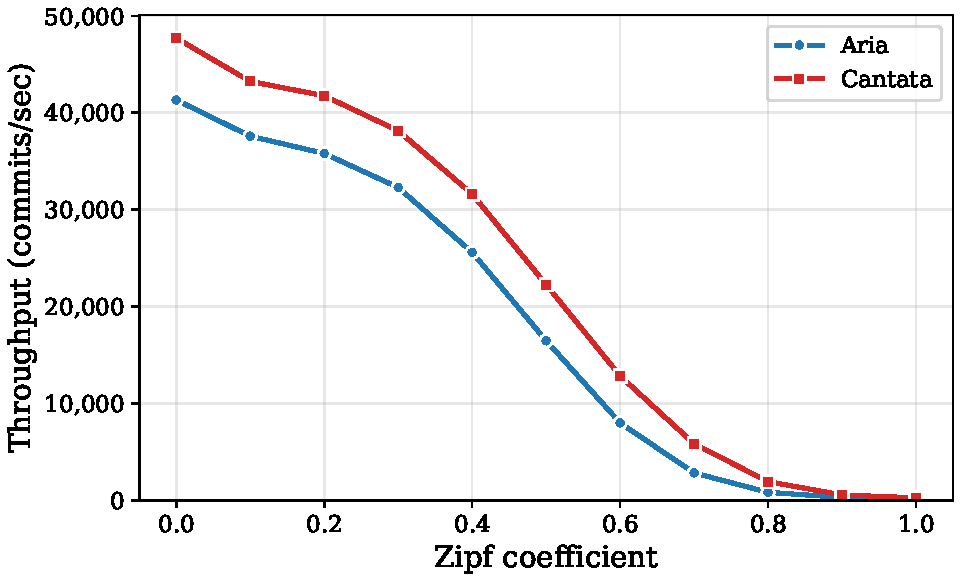
\includegraphics[width=\linewidth]{figure_pdf/medium_high.pdf}
\caption{Throughput comparison under medium-to-high contention (\texttt{read\_write\_ratio}=80, \texttt{ops\_per\_txn}=100, \texttt{batch\_size}=1000). The x-axis represents the Zipf coefficient, and the y-axis represents the average number of commits per second (throughput).}
\label{fig:medium_high}
\end{figure}

We set \texttt{read\_write\_ratio}=80 and \texttt{batch\_size}=1000. Figure~\ref{fig:medium_high} shows the results. Cantata achieved throughput equal to or higher than Aria across all Zipf coefficients. As the Zipf coefficient increased, the throughput gap widened, peaking at approximately 2.4$\times$ near Zipf$\,{=}\,$0.8. Beyond that point the ratio declined, yet Cantata remained consistently superior.

Under moderate contention, WAW dependencies occur frequently enough for Cantata's early detection to effectively suppress false-positive aborts in the subsequent dependency checking stages. Under extremely high contention, however, aborts caused by RAW and WAR dependencies become dominant, and early WAW detection alone cannot absorb all the overhead. Furthermore, the absolute throughput of both methods drops substantially under extreme contention, which narrows the relative ratio.

%%% ---------- Effect of varying batch size ----------
\subsection{Effect of Varying Batch Size}

\begin{figure}[tb]
\centering
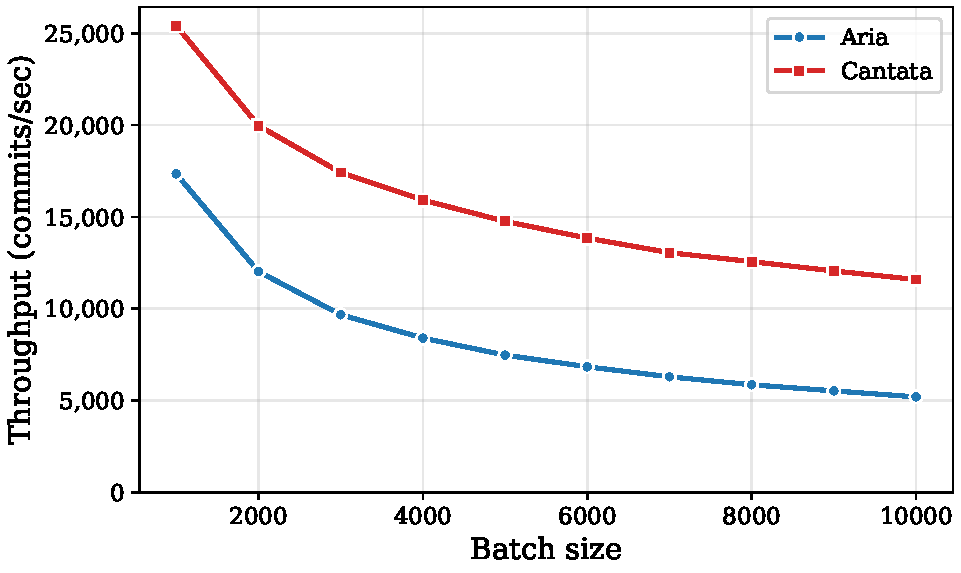
\includegraphics[width=\linewidth]{figure_pdf/vary_batch.pdf}
\caption{Throughput comparison with varying batch size (\texttt{read\_write\_ratio}=95, \texttt{ops\_per\_txn}=100, Zipf$\,{=}\,$0.9). The x-axis represents the batch size and the y-axis represents throughput.}
\label{fig:vary_batch}
\end{figure}

Next, we varied the batch size from 1\,000 to 10\,000 in increments of 1\,000 to investigate how the throughput gap between Aria and Cantata changes as the batch grows larger. Wang et al.~\cite{10.1007/s11704-023-2605-z} pointed out that configuring an appropriate batch size in Aria is a practical challenge, because the optimal batch size depends on workload characteristics. This evaluation also provides insights for future extensions such as adaptive batch sizing.

We set \texttt{read\_write\_ratio}=95 and Zipf$\,{=}\,$0.9, choosing a high read ratio to amplify the effect of Cantata's elimination of unnecessary read reservations.

Figure~\ref{fig:vary_batch} shows the results. The throughput ratio (Cantata/Aria) increased monotonically with batch size, reaching approximately 2.2$\times$ at batch size$\,{=}\,$10\,000. In Aria, the cumulative cost of read reservations and dependency checking for transactions that should be aborted grows as the number of transactions in a batch increases. Cantata skips these downstream operations for transactions whose abort has been determined by early WAW detection, so the benefit of this elimination accumulates further as the batch grows larger.

%%% ---------- Analysis of early dependency resolution and redundant operation elimination ----------
\subsection{Analysis of Early Dependency Resolution and Redundant Operation Elimination}

\begin{figure}[tb]
\centering
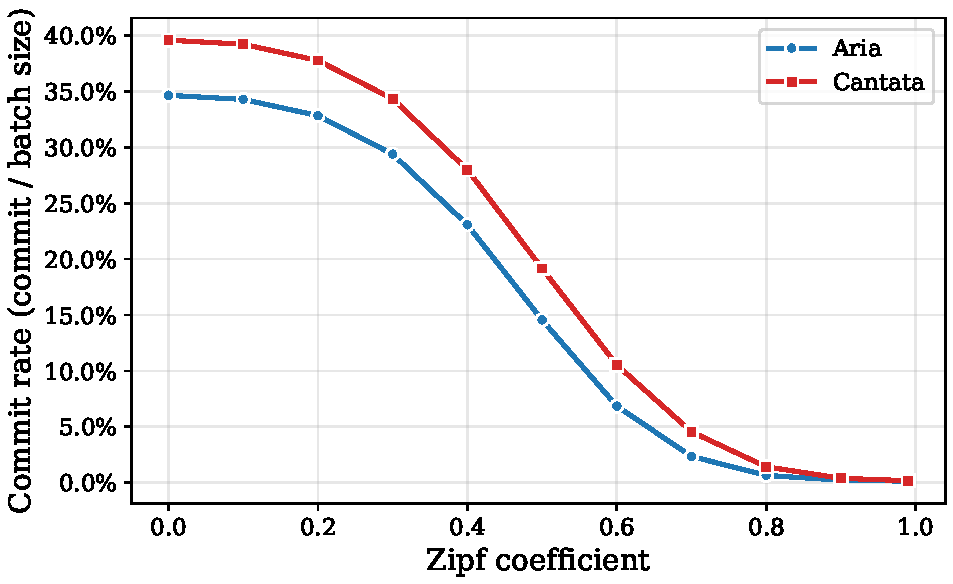
\includegraphics[width=\linewidth]{figure_pdf/commit_rate.pdf}
\caption{Commit rate (committed transactions / batch size) across Zipf coefficients (\texttt{ops\_per\_txn}=100, \texttt{batch\_size}=1000, \texttt{read\_write\_ratio}=80). A higher value indicates that a larger fraction of the batch successfully commits, reflecting a wider scheduling space.}
\label{fig:commit_rate}
\end{figure}

\begin{figure}[tb]
\centering
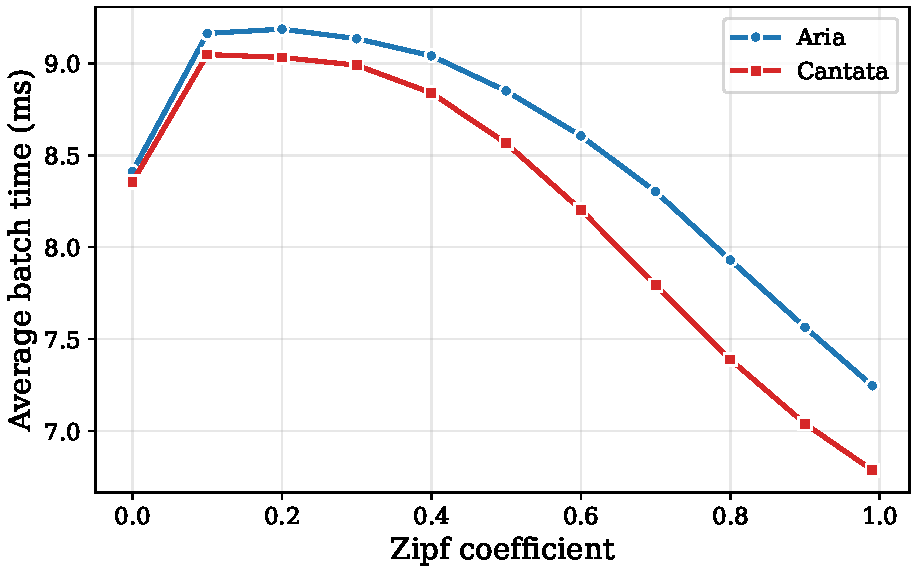
\includegraphics[width=\linewidth]{figure_pdf/batch_time.pdf}
\caption{Average execution time per batch for Aria and Cantata (\texttt{ops\_per\_txn}=100, \texttt{batch\_size}=1000, \texttt{read\_write\_ratio}=80). Each batch covers one complete batch cycle: cleanup, the read phase, and the commit phase.}
\label{fig:batch_time}
\end{figure}

Combining the results from the preceding sections, the throughput improvement of Cantata can be attributed not merely to an increase in the number of committed transactions, but to two underlying effects: the suppression of unnecessary aborts and the elimination of redundant processing for transactions whose abort has already been determined. In this section, we quantitatively analyze these two effects from the perspectives of the commit rate and batch execution time.

\subsubsection{Commit Rate Comparison}

Figure~\ref{fig:commit_rate} shows the commit rate---defined as the average number of committed transactions per batch divided by the batch size---with \texttt{batch\_size}=1000 and \texttt{read\_write\_ratio}=80 while varying the Zipf coefficient. This metric directly represents how large a fraction of the scheduling space each protocol can successfully exploit per batch; a higher commit rate indicates that a wider range of the scheduling space is utilized.
Cantata achieved a higher commit rate than Aria across all Zipf coefficients. As contention increased, both commit rates declined, but Cantata consistently maintained a higher value, committing up to approximately twice as many transactions per batch as Aria under high contention. Under extremely high contention, the gap narrowed because the vast majority of transactions are aborted due to WAW dependencies, leaving very few surviving transactions that can benefit from the expanded scheduling space.

These results demonstrate that Cantata expands the effective scheduling space of Aria. In vanilla Aria, transactions that should be aborted due to WAW dependencies continue to hold their read reservations, which in turn trigger false-positive aborts of other transactions during the subsequent RAW/WAR checking. Cantata detects WAW dependencies early and excludes the affected transactions from downstream processing, thereby suppressing this cascading abort effect and allowing more transactions per batch to commit successfully.

\subsubsection{Batch Execution Time Comparison}

Figure~\ref{fig:batch_time} shows the average wall-clock time per batch, measured using a time-instrumented build. Each measurement covers one complete batch cycle: cleanup, the read phase, and the commit phase.

Cantata exhibited shorter batch execution times than Aria across all Zipf coefficients. The time savings grew with contention, reaching a reduction of approximately 7\% under high contention. This demonstrates that the advantage of Cantata is not solely a consequence of fewer aborts leading to higher throughput; rather, by skipping read reservations and dependency resolution for transactions whose abort has already been determined, Cantata reduces the processing time of each batch itself.

In summary, the performance improvement of Cantata is rooted in two synergistic effects: (1)~the expansion of the scheduling space through early dependency resolution, as demonstrated by the higher commit rate, and (2)~the elimination of downstream processing (read reservations and dependency checking) for transactions whose abort has been determined. These effects become more pronounced as contention increases, and as confirmed in Section~4.5, they accumulate further as the batch size grows larger.

%%% ---------- Ideal-case demonstration of read-reservation skipping ----------
\subsection{Ideal-Case Demonstration of Read-Reservation Skipping}

\begin{figure}[tb]
\centering
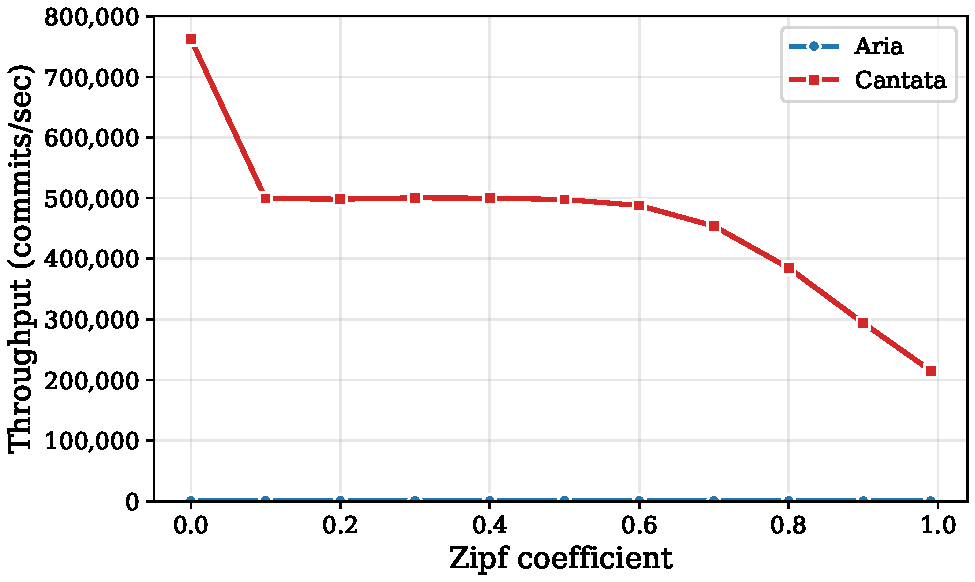
\includegraphics[width=\linewidth]{figure_pdf/sleep_throughput.pdf}
\caption{Throughput comparison in the sleep experiment (\texttt{read\_write\_ratio}=80, \texttt{ops\_per\_txn}=10, \texttt{batch\_size}=1000).}
\label{fig:sleep_throughput}
\end{figure}

The preceding sections have shown that Cantata improves throughput by eliminating redundant read reservations for WAW-aborted transactions.
To isolate this effect, we designed a controlled experiment in which a single transaction's read-reservation phase incurs a 1-second sleep, making the cost of redundant reservations directly observable in overall throughput.

\subsubsection{Experimental Setup}
In each batch of 1000 transactions, the first 25 are designated as \emph{special transactions} that all perform a write to the same data item. Because all 25 share a write target, exactly one special transaction (the one with the smallest TID) commits per batch, while the remaining 24 are aborted due to WAW dependencies and retried in the subsequent batch. Consequently, the 25th special transaction---the one with the largest TID---requires 25 batches before it is the sole remaining special transaction and can finally commit. This 25th transaction is configured to sleep for 1 second during its read-reservation phase.

In Aria, all transactions---including those that will ultimately be WAW-aborted---execute read reservations in every batch. Therefore, the 1-second sleep is incurred in \emph{every} batch until the 25th transaction commits, yielding a cumulative delay of approximately 25~seconds. In Cantata, by contrast, transactions whose abort has been determined by early WAW detection skip the read-reservation phase entirely. The sleep is thus triggered only in the single batch where the 25th transaction finally commits, resulting in a one-time 1-second delay.

\subsubsection{Results}
Figure~\ref{fig:sleep_throughput} shows the throughput of Aria and Cantata in this experiment. Aria's throughput was limited to roughly one thousand commits per second across all Zipf coefficients, confirming that the 1-second sleep dominates the batch duration. Cantata, by contrast, achieved throughput on the order of several hundred thousand commits per second, since the sleep was incurred only once during the entire run. The resulting throughput ratio reached up to approximately 774$\times$.

This result directly confirms Cantata's core mechanism: by detecting WAW dependencies early, Cantata skips read reservations and dependency checking for already-doomed transactions, avoiding the repeated cost that Aria must bear in every batch. In general, as the per-transaction cost of read reservations grows---due to a larger number of read operations or heavier processing per operation---the benefit of this early elimination becomes more pronounced.

%%% ---------- Scalability ----------
\subsection{Scalability}

\begin{figure}[tb]
\centering
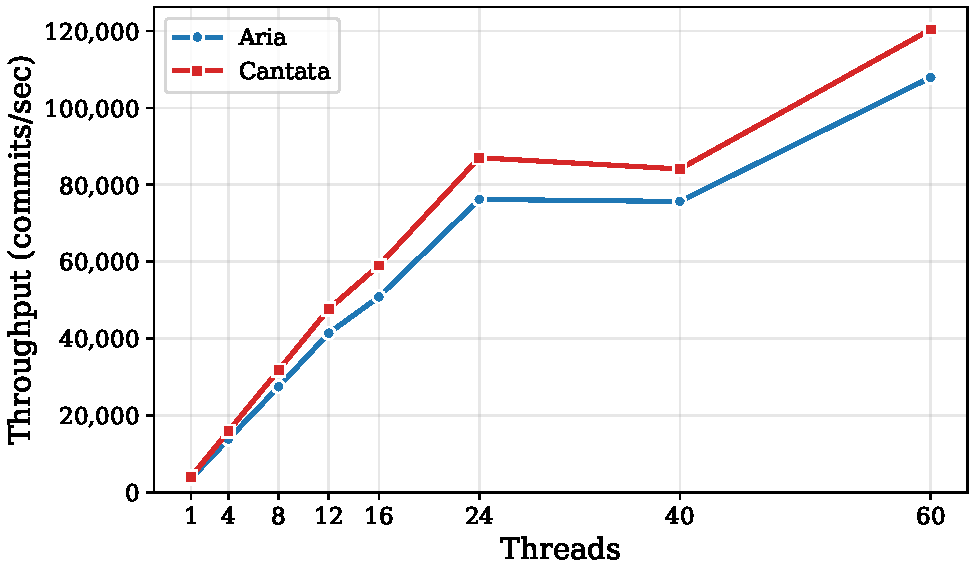
\includegraphics[width=\linewidth]{figure_pdf/vary_thread.pdf}
\caption{Throughput comparison with varying number of threads (\texttt{read\_write\_ratio}=80, \texttt{ops\_per\_txn}=100, \texttt{batch\_size}=1000, Zipf$\,{=}\,$0). The x-axis represents the number of threads and the y-axis represents throughput.}
\label{fig:vary_thread}
\end{figure}

To evaluate scalability, we varied the number of worker threads from 1 to 60 with Zipf$\,{=}\,$0, \texttt{read\_write\_ratio}=80, and \texttt{batch\_size}=1000. Figure~\ref{fig:vary_thread} shows the results. Both Aria and Cantata scaled with the number of threads, and Cantata maintained throughput equal to or higher than Aria across all thread counts. These results confirm that Cantata scales with the number of threads while consistently maintaining throughput equal to or higher than Aria.


\section{Related Work}
\subsection{Deterministic Protocols}
%Calvin \cite{calvin} is a distributed database that employs determinism. In many distributed systems, a two-phase commit method is used, in which the participating nodes agree on a commit. Calvin takes advantage of the characteristics of Determinism, in which the execution results of multiple transactions are attributed to a specific serialization order, to eliminate the two-phase commit bottleneck and achieve high performance.
Aria~\cite{lu2020aria} is a novel deterministic protocol that executes a transaction against a database snapshot and deterministically chooses whether to commit or not at transaction commit time. This flexibility provides novel performance. However, it also may degrade performance due to the limitation of scheduling space incurred by unnecessary transaction aborts.
%

Piece-wise visibility (PWV)~\cite{faleiro17} allows partitioned execution by constructing a dependency graph. By analyzing the dependency, it can execute non-conflicting transactions in parallel. However, conflicting transactions need to be executed one by one, serially. Our proposal does not need expensive graph constructions.
%

%Bohm~\cite{Bohm} is an extension of Calvin and it suffers under skewed workloads during initialization and contention during execution. 
%
%They execute transactions 

Caracal~\cite{qin2021caracal} exploits the epoch concept to increase concurrency in its design. Its scheduling space is conflict serializable, but it exploits multi-version storage. It first creates a version array for each data item in the initialization phase and executes them in the subsequent phase. 
%
The execution of conflicting transactions is in a serial manner, and thus it can be less efficient than Aria.
%
\subsection{Non Deterministic Protocols}
A variety of non-deterministic serializable concurrency control protocols have been proposed to efficiently deal with contended workload.
These protocols work efficiently for short transaction-oriented workloads like YCSB or TPC-C.
%
Some protocols exploit a wide scheduling space~\cite{ermia} based on multi-version based-scheduling space, while conflict serializability-based protocols use a bunch of optimization method exploiting hardware specifications (i.e., NUMA), the decentralization of timestamp generation~\cite{tu2013speedy} or speculative execution~\cite{nakamori2022decentralization,polaris}.
%Bamboo is based on the latter approach and exhibited novel performance for a specific situation that involves hotspots.     
%                                                                       
%To our knowledge, methods to improve the performance of Bamboo has not been addressed prior to our research.
None of these protocols demonstrate efficiency for long-running transaction-oriented workloads.

\subsection{Omittable Writes}
The Thomas Write Rule (TWR)~\cite{10.1145/320071.320076}—originally proposed for timestamp‑ordering (T/O) protocols—allows a system to skip a write issued by an older timestamp if the target record has already been overwritten by a newer one. By discarding such obsolete writes, TWR expands the space of admissible schedules and reduces unnecessary aborts, but its reliance on a global timestamp order limits direct adoption in deterministic OCC engines such as Aria.

Building on TWR, Nakazono et al~\cite{nakazono2019nwr} generalized the idea into the Non‑Visible Write Rule (NWR). NWR replaces the timestamp ordering condition with two semantic conditions: the write must be (i) a blind update and (ii) not the final (most recent) write within the current epoch. When both hold, the operation is provably invisible to all concurrent and future transactions, making it safe to omit. A lightweight, lock-free 128-bit pivot-version object implementation in Silo~\cite{tu2013speedy}, TicToc~\cite{yu2016tictoc} and MVTO~\cite{lim2017cicada} achieved up to 11 × speed‑up on YCSB‑A while adding \verb|<|10\% overhead on TPC‑C, showing NWR’s practicality for write‑heavy workloads.

Because Aria already obtains complete read–write sets and assigns deterministic TIDs within each epoch, integrating NWR would likely require only an additional simple check (e.g., blind $\land$ earliest assigned transaction ID within the epoch) before the commit phase.
Although we have begun preliminary exploration into combining Aria and NWR, a rigorous validation of the exact conditions and potential further optimizations remains an open issue for future research. Improving or relaxing this condition could possibly yield even higher performance gains, which is a promising direction that merits additional investigation.



%%%%%%%%%%%%%%%%%%%%%%%%%%%%%%%%%%%%%%%%%%%%%%%%%%%%%%%%%%%%%%%%%%%%%%%
\section{Conclusion}
Aria, a deterministic concurrency control protocol, generates unnecessary aborts and redundant operations because it checks all dependencies at once. This paper proposed Cantata, an optimization that reduces these inefficiencies through early dependency resolution, which divides dependency checking into two stages. Experiments under high contention showed that Cantata achieved higher throughput than Aria. Furthermore, in experiments with long-running transactions, Cantata achieved up to 774$\times$ higher throughput than Aria. A controlled experiment that artificially amplified the cost of a single redundant read reservation confirmed that Cantata's advantage stems from skipping subsequent operations for WAW-aborted transactions. These results indicate that Cantata is less susceptible to delays caused by aborted transactions with long read operations, and that the benefit of early dependency resolution grows with the per-transaction cost of redundant operations.

\section*{Acknowledgments}
This paper is based on results obtained from the project "Research and Development Project of the
Enhanced Infrastructures for Post-5G Information and Communication Systems (JPNP20017) " and
JPNP16007 commissioned by the New Energy and Industrial Technology Development Organization
(NEDO), and from JSPS KAKENHI Grant Number 22H03596, and from JST CREST Grant Number JPMJCR24R4 and from SECOM Science and Technology Foundation and JST COI-NEXT SQAI (JPMJPF2221).

\def\newblock{\hskip .11em plus .33em minus .07em}
\bibliographystyle{ipsjunsrt}
\bibliography{edr}


\end{document}
